\documentclass{report}
\usepackage{framed}
\usepackage[outerbars]{changebar}

% Dimensions de la page
\usepackage{geometry}
%\geometry{scale=0.8}
\geometry{a4paper}

% Acronyms
\usepackage[nonumberlist]{glossaries}
\setacronymstyle{long-short}
\makenoidxglossaries
% Load acronyms list
\loadglsentries{../acronyms}

% Graphics
\usepackage{graphicx}
\graphicspath{{../Figures/Generating_music/Hexahedria/}}

% Prettyref
\usepackage{prettyref}
\usepackage{hyperref}

\title{Music generation review}
\author{Aciditeam}
\begin{document}
\maketitle

\section{HMM}
HMM-based models have been widely used for harmonic structure analysis \cite{allan2005harmonising,pickens2003polyphonic,pachet2001musical} or melodic composition \cite{Yamanishi:2010aa}, but not for polyphonic composition. Indeed, HMM are not well-suited for multi-dimensional data and, thus, remained targeted at monophonic or chord sequences. In harmonization models (\cite{allan2005harmonising}), an interesting "root relative" representation is used. Each note is represented by its distance to the root (given the key), while a chord label is added to indicate the harmonic context of the chord (its degree).

\gls*{HMM} are a particular case of \gls*{MRF}, and Lavrenko proposed to use a less constrained lattice of binary units directly derived from the piano-roll representation\cite{lavrenko2003polyphonic}. Here, the time structure is eluded by only considering the notes onset, while removing their duration. The efficiency of such an under-defined representation can be doubted, but it offers a first easy-to-handle representation. Intuitively, this representation might perform well on music strictly aligned on a temporal grid such as Bach's chorales. Besides, pitches are reduced to 12 through an octave-equivalent transformation. This transformation (named \textit{pitch-class transformation} here) is interesting as it can help the system focusing on the harmonic structure of music.
The field is built on \textit{directed} temporal connection, which is a reasonable assumption that only notes played in the past influence notes in the future. A more surprising and restrictive assumption is that a certain pitch is only influenced by lower pitches at the same time. The distribution of the field is defined through a set of feature functions and parameters, representing rules learned on a training dataset.

Several works are based on \gls*{RBM}, such as systems that automatically creates Jazz melody over a sequence of chords \cite{bickerman2010learning}. Here, a data representation well fitted for their problem is to perform a separate representation of chords and melodies. However the poor temporal structure (simple concatenation of successive frames) of their system appears as an immediate limitation. Very recently, two models aimed at automatic music generation specifically targeted the temporal dimension and were able to generate interesting music sequences.

\section{RNN-RBM}
\subsection{Data representation}
Pianoroll
\subsection{Model}
\begin{figure}
\centering
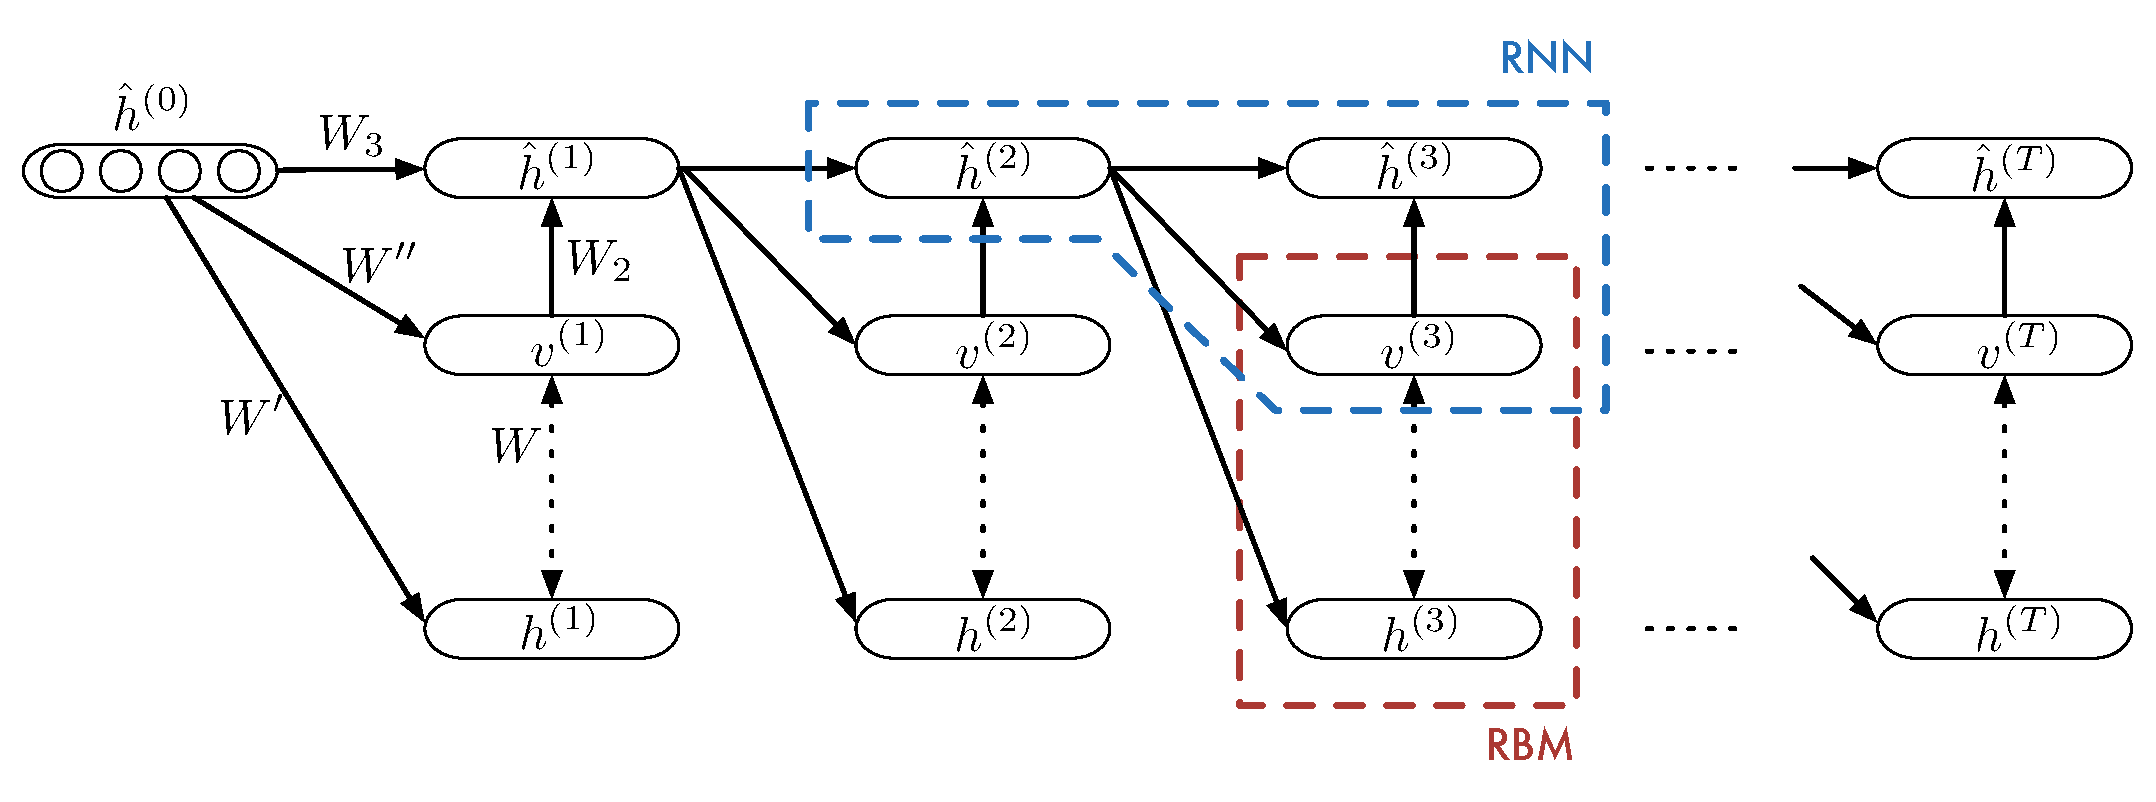
\includegraphics[scale=0.4]{RNN-RBM}
\caption{Graphical structure of the RNN-RBM. We can distinguish the two parts of the model, RNN in blue and RBM in red.}
\label{fig:RNN-RBM}
\end{figure}
A first paper \cite{boulanger2012modeling} introduces two models with a temporal component used to produce polyphonic music sequences : the \gls*{RTRBM} and the \gls*{RNN-RBM} (see \prettyref{fig:RNN-RBM}). Those two models have been inspired by the aforementioned text-generative model \cite{sutskever2011generating}. Beside, an interesting evaluation framework is proposed in this article and will be used to evaluate the performances of our model (\prettyref{sec:music_prediction}).
The general definition of a \gls*{TRBM} introduced by \cite{sutskever2009recurrent} is a sequence of \gls*{RBM} where each \gls*{RBM} is conditioned by the previous one. It can be seen as a HMM with an exponentially large state space (increases with $N^{t}$) but a compact parametrization (only 2 transition matrices and biases). In fact, in the simplest \gls*{TRBM}, only the bias of the hidden units is affected by the previous hidden unit.

The probability of a sequence of observation is given by
\begin{equation}
P(v_{1}^{T},h_{1}^{T}) = P_{0}(v_{1},h_{1}) . \prod_{t=2}^{T} P(v_{t},h_{t}|h_{t-1})
\end{equation}
which is the equation of an HMM, and where the conditional distribution $P(V_{t},H_{t}|H_{t-1})$ is the distribution of an \gls*{RBM} whose hidden bias $H_{t}$ is a function of $h_{t-1}$ (named \textit{dynamic bias}).
\begin{equation}
P(v_{t},h_{t}|h_{t-1}) = exp(v_{t}^{\top}b_{V} + v_{t}^{\top} W h_{t} + h_{t}^{\top}(b_{H} + W'h_{t-1})
\end{equation}
The main difference between the \gls*{RNN-RBM} model and the \gls*{RTRBM} is that the recurrent relation is based on the mean-field values of the hidden units instead of their binary values. Hence, those mean-field values units are separated from their binary alter ego and define another set of weights that models the recurrent relations.
A \gls*{RNN-RBM} can be trained using the \gls*{BPTT} algorithm \cite{rumelhart1985learning}.

\section{Long Short-Term Memory (LSTM)}
\subsection{Data representation}
Pianoroll
\subsection{Model}
The paper \cite{eck2008learning} addresses blues improvisation by proposing a model based on a slightly modified Long Short-Term Memory (LSTM) network \cite{eck2002finding}. More precisely, their model is composed of an input layer, an output layer, and a hidden layer made of a standard feed-forward layer in parallel with several LSTM blocks, and use the same aforementioned evaluation framework \cite{DBLP:journals/corr/LiuR14a}.
\begin{figure}
\centering
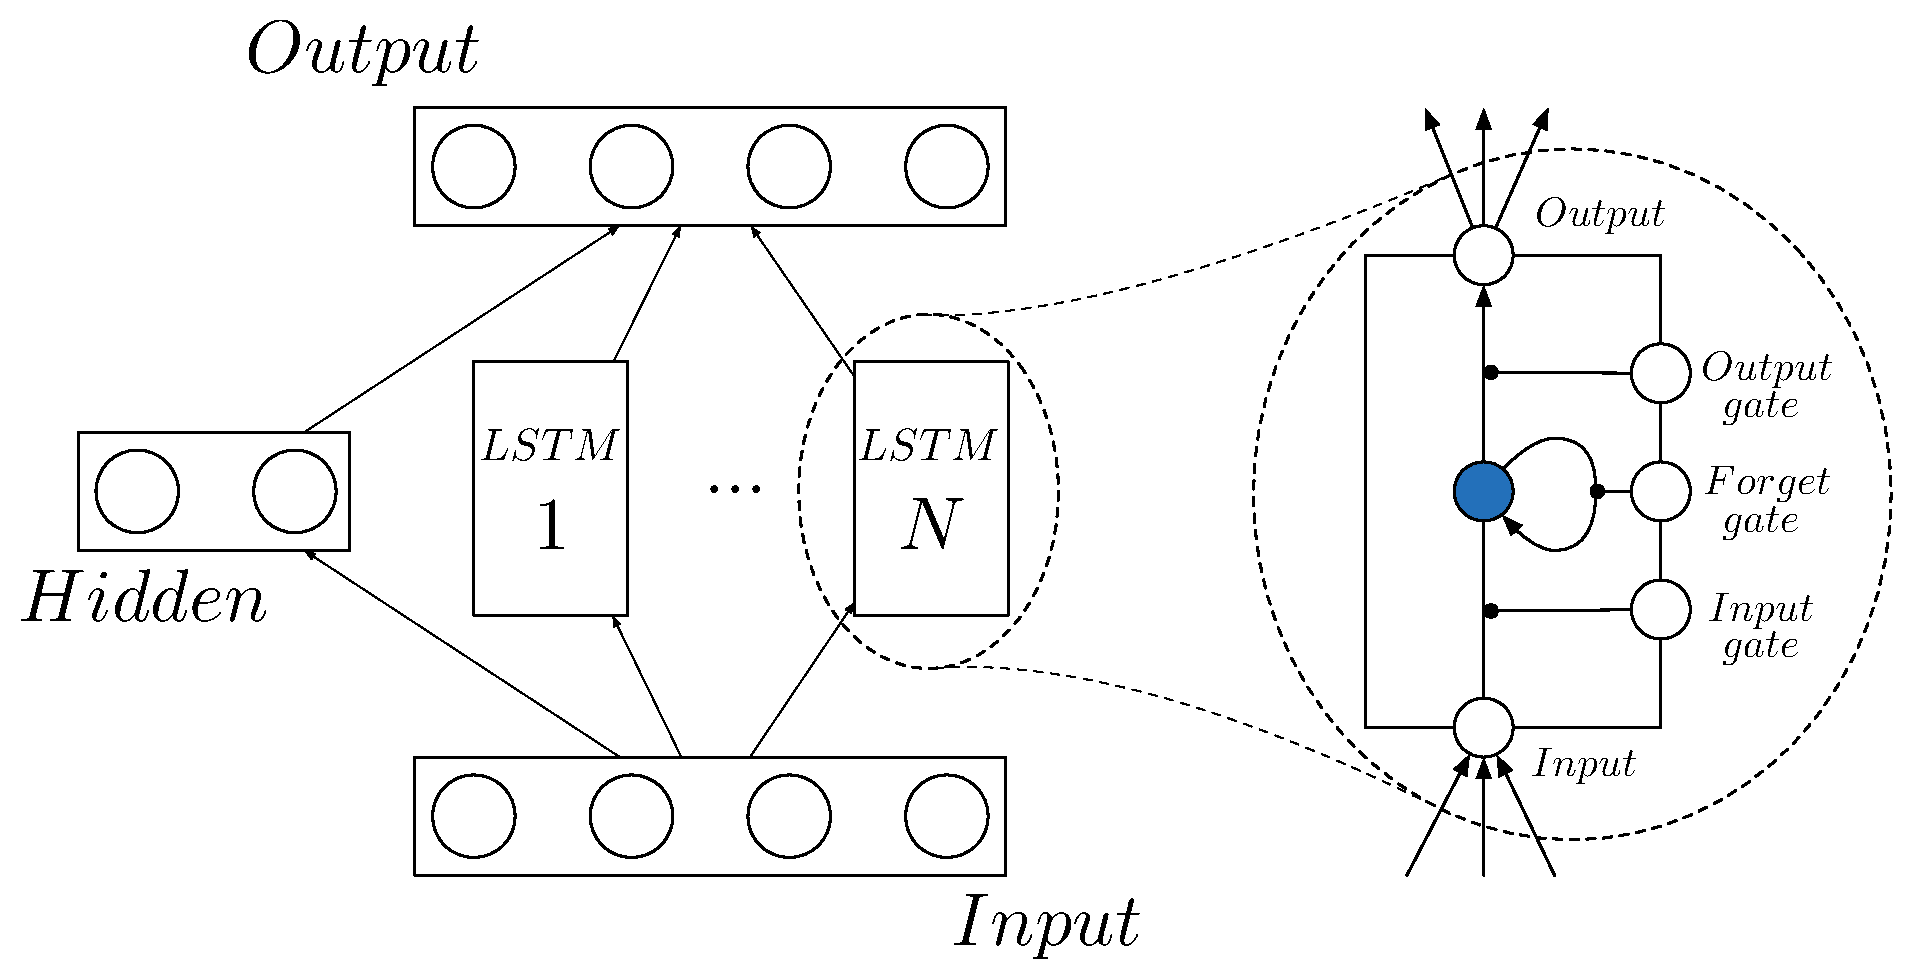
\includegraphics[scale=0.5]{LSTM_music}
\caption{The modified LSTM model used in \cite{eck2008learning}. The hidden layer is a standard feed-forward layer in parallel with }
\label{fig:LSTM_music}
\end{figure}
A \textit{LSTM} block in a network plays the same role as any other computational unit (they compute a single output value from weighted inputs), but have a more complex structure.
Since the generation process is a random selection, very unlikely musical event can still happen. Even if we want to keep a certain amount of randomness in our generative process, we still don't want those very unlikely event to happen. To do so, a threshold is applied before sampling from the output distribution in order to avoid very low probability notes to be chosen.

\section{Hexadria (RNN-based architecture)}
\begin{figure}
\centering
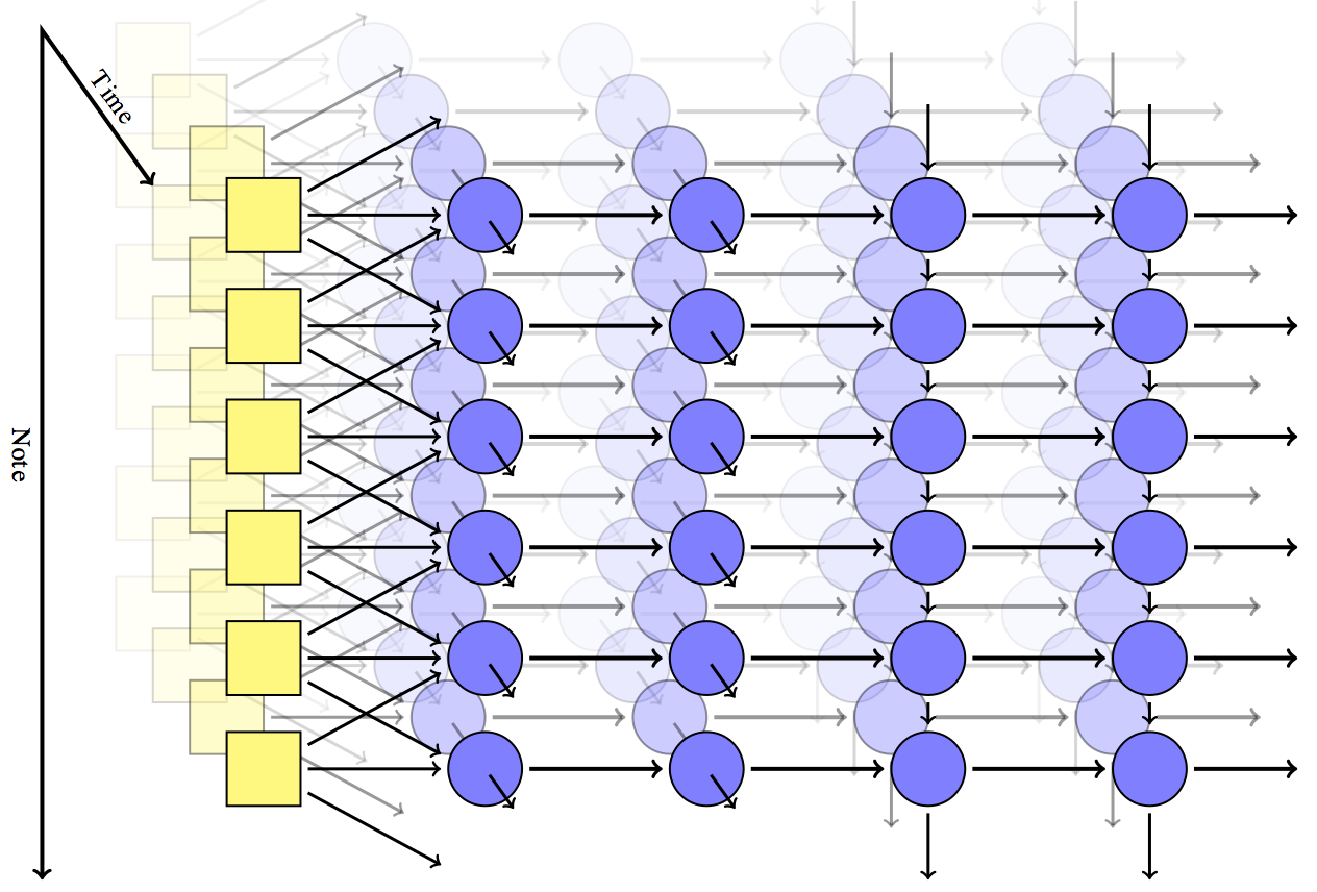
\includegraphics[width=0.45\linewidth]{RNN_convol_hexadedria}
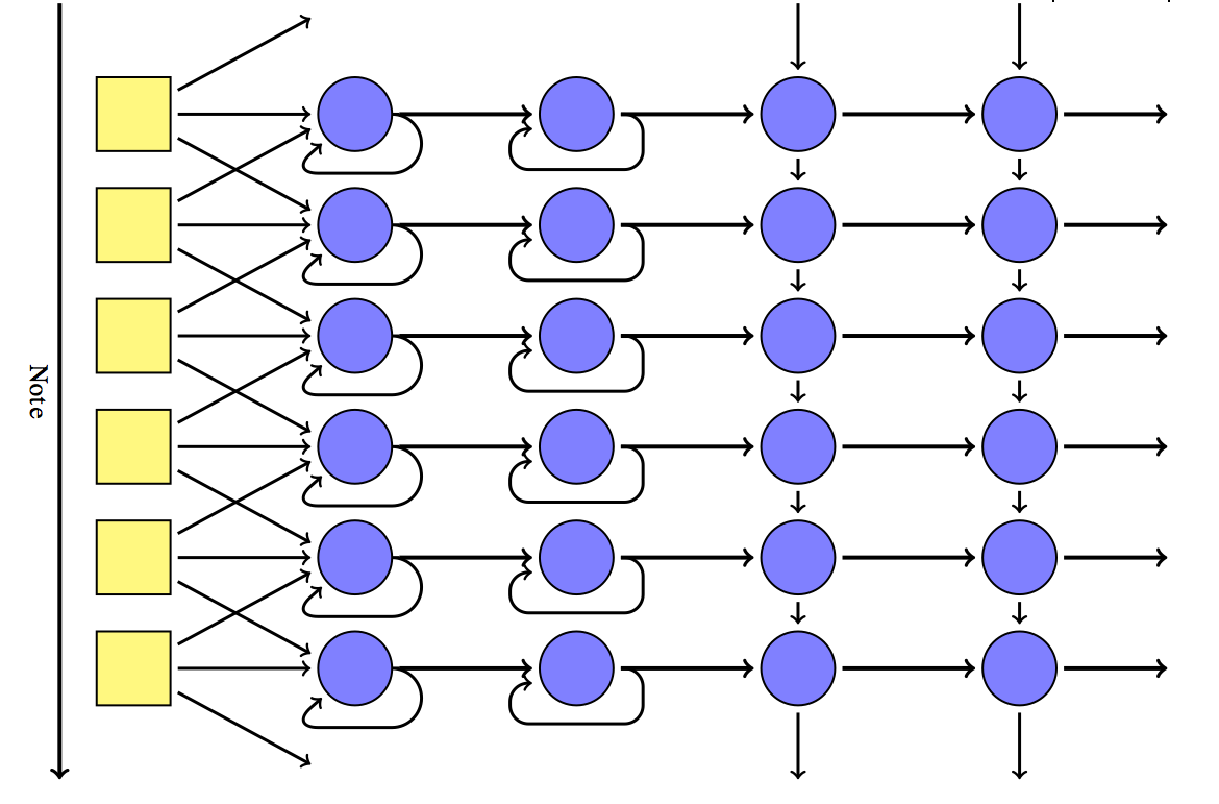
\includegraphics[width=0.45\linewidth]{RNN_convol_hexadedria_2}
\caption{Convolution RNN. The same little network is associated to each note (convolutive network). In upper layers, thos network have \textit{lateral} connection.}
\label{RNN-hexadria}
\end{figure}
\subsection{Data representation}
See article for details, but input are described by a pitch-class (12) and an position unit (1, binary between melody and chords). The previous time frame is encoded by two vectors : \textit{previous vicinity} and \textit{previous context}. \textit{Previous vicinity} is a plus/minus octave vector with an information about whether or not the not has been \textit{articulated}, i.e. repeated and not sustained. This is the voice leading information. This past information is reinforced by a \textit{previous context} vector which is simply a vector of length 12 containing the sum of the note per pitch-class present in the previous time step. This is more an harmonic information.
A \textit{beat} information is added (dim 4), which give the information of the place of the current frame in a 4/4 measure. Which is fucking clever.
At the end of each "pitch-level" (row in the figure \prettyref{RNN-hexadria}), which represent a note, a play probability and an articulate probability is outputted.

\subsection{Model}
Proposed by Daniel Johnson (no paper, only a well documented website \href{hexadria}{http://www.hexahedria.com/2015/08/03/composing-music-with-recurrent-neural-networks/}, 2015). 
"The solution I decided to go with is something I am calling a “biaxial RNN”. The idea is that we have two axes (and one pseudo-axis): there is the time axis and the note axis (and the direction-of-computation pseudo-axis). Each recurrent layer transforms inputs to outputs, and also sends recurrent connections along one of these axes. But there is no reason why they all have to send connections along the same axis!"
"Notice that the first two layers have connections across time steps, but are independent across notes. The last two layers, on the other hand, have connections between notes, but are independent between time steps. Together, this allows us to have patterns both in time and in note-space without sacrificing invariance!"
Note that the two last layers on the figure don't have temporal connections.

\subsection{Results}
Impressive. Best so far.
\end{document}